\chapter{Concept}
\label{s:concept}
As explained in the previous chapter, conventional dew point hygrometers used in industry and science, achieve their high degree of accuracy and stability through their rather complex structure, which results in a high cost and large system size. The following section describes the techical structure of common dew point mirror hygrometer designs  and gives an overview of the changes made in order to be able to achieve a reduction in system size and cost while still maintaining accuracy.

\section{Chilled mirror dew point hygrometer}

\begin{figure}[bt]
    \centering
    \input{drawings/text34.pdf_tex}
    \caption{Typical structure of a chilled mirror dew point hygrometer. LEDs emit light onto a mirror surface. Changes in dew formation are detected by a comparison to a reference signal.}
    \label{d:hygrometer}
\end{figure}


As shown in \cref{d:hygrometer}, the typical structure of a dew point mirror hygrometer contains three main parts: 
\begin{itemize}
    \item the optical system consisting of light emitters, light detectors and a mirror,
    \item the cooling system, regulated using the feedback of the optical system,
    \item the temperature readout
\end{itemize}

\subsubsection{Mirror}\label{s:mirror}
Core to the system is the chilled mirror, which surface needs to be sensed with regards to the prevalence of condensed or deposited water vapor and the temperature that is prevalent during the process. While the surface may consist of different kind of materials, it is important that dew can readily form and that there is a subsequent change in refraction or scattering in response to the changed conditions. In literature, different kind of materials with a varying detail in their specification have been used for studied devices, ranging from conventional coated glass substrate mirrors to bare metals like copper or gold. Depending on the used type, properties such as wavelength-dependent refraction, thermal conductivity and mass, corrosiveness and likelihood of vapor formation can differ. The refraction indices of gold and copper for example are much lower for visible light than for infrared radiation, indicating that the type of material should also take the intended light source of the system into account and vice versa. Calculations of the intensity of scattered light depending on the roughness and incident direction as performed in a study of Matsumoto and Toyooka show, that while smooth surfaces with an average roughness of \qty{0.1}{\micro\m} have high relative refractive loss in response to dew, this loss is only to be seen at a scattering angle close to the incident angle, possibly requiring a more precise positioning of light source and detection, but in turn yielding optimal optical response. Surfaces with a higher average roughness of \qty{1.0}{\micro\m} and \qty{2.0}{\micro\m} generally scatter incident light much more, leading to two respectively three order of magnitudes lower light intensities at same refraction angles, but may have benefits on the formation of dew \autocite{matsumotoDeterminationDewPoint1992a}.
\\

\subsubsection{Light emitter and detector}
\begin{wrapfigure}{r}{0.55\textwidth}
    \centering
    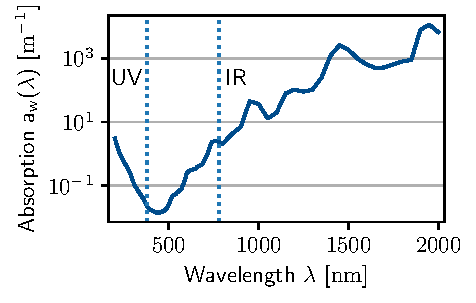
\includegraphics{graphs/waterabsorption.pdf}
    \caption{Electromagnetic absorption by liquid water based on data from \autocite{aasVerticalTransferInfrared2006,smithOpticalPropertiesClearest1981}.}
    \label{g:waterabsorption}
    % \vspace{-10pt}
\end{wrapfigure}
Light emission is usually performed using laser systems, such as vertical cavity surface emitting lasers, or LEDs \autocite{chenHumiditySensorsReview2005,sweeneySemiconductorLasers2017}. While for each system, different options in wavelengths are possible, a commonly used spectrum is the lower range of the near infrared band, which ranges between \qtyrange{780}{2500}{\nano\m} . The reasons for this is two-fold: On the one hand light sources in this spectrum are readily available in various form factors and power outputs at low cost and on the other hand, water molecules are exhibiting a significantly higher absorption in the infrared region of the electromagnetic spectrum than in the visible spectrum and the upper region of the ultraviolet spectrum as seen in \cref{g:waterabsorption}. The light source can either emit directly onto the mirror surface or be used in conjunction with an optical system, such as lenses or glass fibers in order to allow for a greater degree of control.

The most commonly used optical sensing devices are photoresistors and photodiodes, which employ the photoconductive and photovoltaic respectively. Both effects are found in semiconductors. Photoresistors are based on the phenomenon, that certain semiconductive materials form electron-hole pairs in case of incident photons with an energy higher than the band gap energy, thus leading to a change in conductivity. Photodiodes consisting of a p-type and n-type semiconductor employ the principle of a change in charge distribution due to the formation of electron-hole pairs in case of incident light, resulting in a voltage across the junction, which is proportional to the amount of said light.
In research, most optical dew point sensors are using photodiodes as for their much higher spectral response in the relevant wavelengths \autocite{kumeOpticalDetectorsReceivers2017}.


% \LENGTHDIVIDE{\textwidth}{1mm}{\size} 
% \size    
\clearpage
\subsubsection{Cooling system}\label{s:peltier}
\begin{wrapfigure}{r}{0.43\textwidth}
    % \centering
    % \def\svgwidth{\textwidth}
    \input{drawings/peltier.pdf_tex}
    \caption{Structure of a TEC. Heat is transferred depending on the direction of current.}
    \label{d:peltier}
\end{wrapfigure}

The cooling of the mirror is often performed using a thermoelectric cooler, which uses the Peltier-effect, discovered by Jean Peltier in 1834, which is a thermoelectric phenomenon where a temperature difference is created by applying a voltage between two electrodes connected to a semiconductor material. In a thermoelectric cooler (TEC), also known as Peltier device, DC current flows through the device causing heat to be transferred from one side to the other, creating a temperature difference as shown in \cref{d:peltier}. The device consists of p-type and n-type semiconductor blocks connected electrically in series and thermally in parallel. When current is passed through the device, charge carriers (electrons in n-type and holes in p-type materials) move and carry heat with them, absorbing heat at the cold junction and releasing it at the hot junction. The heat transfer rate of the TEC increases with current up to a certain point, after which it becomes linear even as current continues to increase. The maximum temperature difference that can be achieved depends on factors like the properties of the semiconductor materials used and the geometry of the device. Compared to vapor-compression refrigeration TECs have the advantages of fine temperature control, small size and lack of moving parts, however at the cost of a low efficiency of a less than \qty{20}{\percent} \autocite{caiThermoelectricCoolingTechnology2019a,zhangThermoelectricMaterialsEnergy2015}.

The response of a TEC to an applied current is not instantaneous, but rather exponential with a time constant mainly dependent on the heat capacity of the ceramic substrate and usually in the range of seconds. In order to obtain faster measurements, additional heat can be introduced, e.g. by reversing the direction of current in the TEC \autocite{pascal-delannoyFastHumiditySensor1998}

\subsubsection{Temperature readout}
During the process of cooling the mirror and sensing the formation of dew or frost, the temperature of the mirror has to be constantly monitored for detection and control purposes. In literature, the two most commonly used types of sensing devices are  \glspl{RTD} and thermocouples. 

 \glspl{RTD} are precision temperature sensors that exploit the predictable change in electrical resistance of materials with temperature. The most common  \gls{RTD} materials include platinum, nickel, and copper, with platinum  \glspl{RTD} offering the highest accuracy and long-term stability. In case of platinum  \glspl{RTD}, the accuracy is standardized into classes according to IEC 60751, with class AA specifying the most accurate results of \qtylist{\pm 0.1}{\celsius}, however for even higher requirements,  \glspl{RTD} with an even higher precision are available. In order to guarantee the accuracy, these devices rely on a well designed measuring circuit in order to mitigate effects of lead resistance \autocite{wuBasicGuideRTD2018}.

Thermocouples consist of two dissimilar metals joined together at their ends. When a temperature gradient exists between the junctions, a voltage is generated due to the Seebeck effect, the inverse of the previously described Peltier effect. The magnitude of this voltage is proportional to the temperature difference between the hot and cold junctions. Commonly used types of metals are iron-constantan (Type J), chromel-alumel (Type K) and copper-constantan (Type T), with the latter allowing for most precise measurements with an accuracy rated up to \qty{\pm 0.5}{\celsius}.

The quality of measurement also depends on placement of the sensor, optimally directly embedded into the mirror in close proximity to the sensing area \autocite{hallAdvancementsMeasurementUncertainties2016}.




\section{Proposed design}
The aim of this work as stated in \cref{s:introduction} is to create a system, that can provide accurate measurements while employing a simple structure in order to achieve an affordable and reliable solution for precise measurements. To achieve this, three key components for improvement have been determined: usage of integrated off-the-shelf sensing devices as used in the billions in consumer electronics, easily manufacturable and small structures. 

The first concept tried to build on aforementioned designs of well-researched dew point mirror hygrometers. Key distinctions of the concept analyzed throughout this work are the following: 
\begin{itemize}
    \item Usage of a \gls{ENIG} coated copper plane on a \gls{FPC}.
    \item Integrated temperature sensors mounted in close proximity of the sensing area and with a electrical and thermal connection on top of the metallic mirror.
    \item Measurement of dew or frost by the means of a proximity sensors as used in consumer electronics.
\end{itemize}


\begin{figure}[h!]
    % \begin{wrapfigure}{l}{0.6\textwidth}
        \centering
        % \def\svgwidth{\textwidth}
        \input{drawings/concept_build.pdf_tex}
        \caption{Simplified design proposal. Bottom PCB (green) incorporates two kinds of proximity sensors (four in total). Top FPC (blue) has a ENIG-plated mirror on its bottom side, with part of the area used for a planar, interdigital capacitive sensing element, alongside four temperature sensors directly placed and distributed on the area. On its top side, a TEC sits directly above coiled heater traces (not shown here) for thermal control of the mirror/capacitor surface.}
        \label{d:concept_build}
    % \end{wrapfigure}
\end{figure}

As described in \cref{s:mirror}, gold is a very suitable material for optical sensing of infrared radiation due to its high refractive loss in response to dew. The deposition method \Gls{ENIG} is widely used throughout the electronic industry due to its advantages, such as oxidation resistance due to its denser crystal structure compared to electroplated gold, as well as surface planarity and softness leading to good solderability \autocite{shahNovelElectrolessNickel2019}. As a mirror material it is of particular interest, as there is no need for electroplating, providing cost benefits, while enabling soldering of miniature sensors on the surface.

Temperature sensors used in dew point hygrometers employ traditional platinum resistors or thermocouples. Although proven technology, \glspl{RTD} require careful design of the resistance measurement circuitry, while thermocouples are much less accurate and additionally much less linear. Integrated temperature sensors have evolved to be accurate sensing devices, employing ratiometric measurement of the temperature by comparing a voltage proportional to absolute temperature with the quasi-constant bandgap reference voltage. However, the temperature range more limited, typically ranging between \qtyrange{-55}{125}{\celsius} and calibration performed at not more than one temperature \autocite{pertijsPrecisionTemperatureSensors2006}.

Proximity sensors are widely used in consumer electronics, providing a cheap and reliable method in sensing the distance to an object. In their commonly available form, they provide all necessary components to emit light in the desired wavelengths and means for accurate sensing 
\autocite{chapronHighlyAccurateBathroom2020a,umMultipleIntensityDifferentiation2011a}.

While the changes are rather subtle, their successful application in the field of hygrometry would allow for a greatly reduced part count in the construction of the dew point sensor as costly components such as optics, accurate resistive temperature devices and complex readout circuits are avoided with a simultaneous improvement in manufacturability due to avoiding custom setups of lens and mirror configurations.

During the evaluation and improvement of the initial design, a second concept based on capacitive dew detection was implemented. In order for dew being able to form, the capacitive sensor requires a sufficiently large and unobstructed interface to the sampled air volume. For a sufficiently high resolution, the change in capacitance as a result of condensed or deposited water vapor.


% \section{Similar work}
% Investigated similar works focus mainly on dew point sensing hygrometers. For a brief overview of other concepts please refer to section \cref{s:hygrometertypes} and literature \autocite{chenHumiditySensorsReview2005,fontesHumiditySensors2005,korotcenkovHandbookHumidityMeasurement2019}.

% This work is based on other studies on dew point mirror hygrometers, which have different particular topics, such as response time, rough mirror surface conditions, optical enhancements such as the use of glass fibers or robustness in the harsh conditions of upper atmosphere.

% A study exploring capacitive dew point measurement is ... using printed PCBs, achieving TODO. TODO use a quartz crystal oscillator in order to detect. Other studies explore micromachined optical sensors for a planar measurement of dew.
